% Created 2020-07-13 Mon 10:34
% Intended LaTeX compiler: pdflatex
\documentclass[presentation]{beamer}
\usepackage[utf8]{inputenc}
\usepackage[T1]{fontenc}
\usepackage{graphicx}
\usepackage{grffile}
\usepackage{longtable}
\usepackage{wrapfig}
\usepackage{rotating}
\usepackage[normalem]{ulem}
\usepackage{amsmath}
\usepackage{textcomp}
\usepackage{amssymb}
\usepackage{capt-of}
\usepackage{hyperref}
\usetheme{UoB}
\author{Mark Blyth}
\date{\textit{[2020-07-13 Mon]}}
\title{Periodic splines discretisation}
\hypersetup{
 pdfauthor={Mark Blyth},
 pdftitle={Periodic splines discretisation},
 pdfkeywords={},
 pdfsubject={},
 pdfcreator={Emacs 26.3 (Org mode 9.1.9)}, 
 pdflang={English}}
\begin{document}

\maketitle

\section{Background}
\label{sec:org9672594}
\begin{frame}[label={sec:org0d0e1db}]{Week's activities}
\begin{itemize}
\item Finish manuscripts
\begin{itemize}
\item Paper in progress
\begin{itemize}
\item Proposed edits completed
\item Word-count down to 6050+400
\end{itemize}
\item Abstract done
\end{itemize}
\item Read about numerical continuation discretisation
\item Read up on non-Bayesian splines
\item Started periodic splines discretisation
\end{itemize}
\end{frame}

\section{The new work plan}
\label{sec:orgbb37f26}
\begin{frame}[label={sec:orge86ca2c}]{Conference paper goals}
Two separate-but-related goals:
\vfill
\begin{enumerate}[<+->]
\item Demonstrate the use of surrogate modelling
\begin{itemize}
\item Fancy \emph{[adaptive]} filtering; removes noise but not signal
\item Useful for applying Fourier \emph{[wavelets?]} to noisy signals
\item Can produce a statistically optimal noise removal, which traditional filtering does not
\end{itemize}
\item Discretise multiple-timescale signals
\begin{itemize}
\item Fourier gives overly-high-dimensional discretisations on spiking signals
\item Demonstrate an alternative \emph{[lower-dimensional]} method
\item Use simple standard methods to do so
\end{itemize}
\end{enumerate}
\end{frame}

\begin{frame}[label={sec:org1156a9f}]{Surrogate modelling}
This part is done, doesn't require much work
\vfill
\begin{itemize}
\item Previous work on GPR, BARS
\item Shows how to reconstruct a signal from noisy observations
\begin{itemize}
\item Alternative to low-pass filter, that works on spiking signals
\end{itemize}
\item Useful for applying Fourier to noisy signals
\begin{itemize}
\item Removes noise
\item \alert{No Nyquist cap}
\end{itemize}
\end{itemize}
\end{frame}


\begin{frame}[label={sec:org2bc490a}]{New discretisation}
Part (1) let us use Fourier on noisy signals, but discretisation will be high-dimensional
\begin{itemize}[<+->]
\item Collocation etc. requires an ODE model; inapplicable, even on surrogates
\begin{itemize}
\item Find polynomials that solve ODEs at points on orbit
\item Track a point on an orbit; point on orbit + ODE model = full orbit
\item We need more -- need to track the full orbit \emph{without} a model
\end{itemize}
\item Discretisation is just some lower-dimensional representation of a signal
\begin{itemize}
\item Eg. parameters of a regression model that reconstructs the signal
\item Complex method: coefficients of Bayesian periodic splines, or inducing points of sparse periodic GPR \emph{[previous work]}
\item Simple method: coefficients of \emph{[non-Bayesian]} periodic splines \emph{[new work]}
\end{itemize}
\item NODYCON discretisation method: \emph{[non-Bayesian]} periodic splines
\end{itemize}
\end{frame}

\section{Periodic splines}
\label{sec:org0b6d992}
\begin{frame}[label={sec:orgebfd0bd}]{Periodic splines}
Simple non-parametric method for periodic signals
\vfill
\begin{enumerate}[<+->]
\item Find the period
\begin{itemize}
\item Autocorrelation or nonlinear least squares \(F_0\) estimation
\item Fourier?
\end{itemize}
\item `Stack' periods
\begin{itemize}
\item Re-label data \(t_i\)s to phase \(\phi_i = \frac{t_i}{T} \mod 1\) or \(\phi_i = t_i \mod T\)
\end{itemize}
\item Build splines model
\begin{itemize}
\item Discretisation = BSpline coefficients
\end{itemize}
\end{enumerate}
\end{frame}

\begin{frame}[label={sec:orgd3ebd17}]{Period stacking}
Uses ACF to estimate frequency, then NLS to refine estimate

\begin{center}
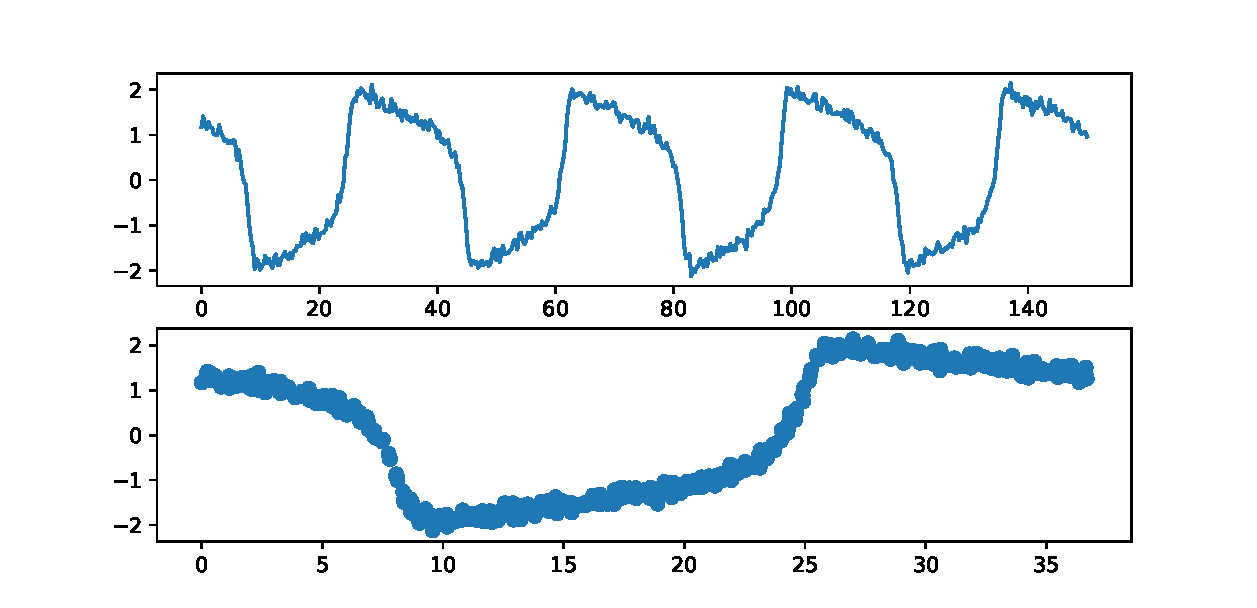
\includegraphics[width=.9\linewidth]{./period_stack.pdf}
\end{center}
\end{frame}

\begin{frame}[label={sec:orge347f9e}]{Period stacking}
Uses ACF to estimate frequency, then NLS to refine estimate; removes period from continuation scheme

\begin{center}
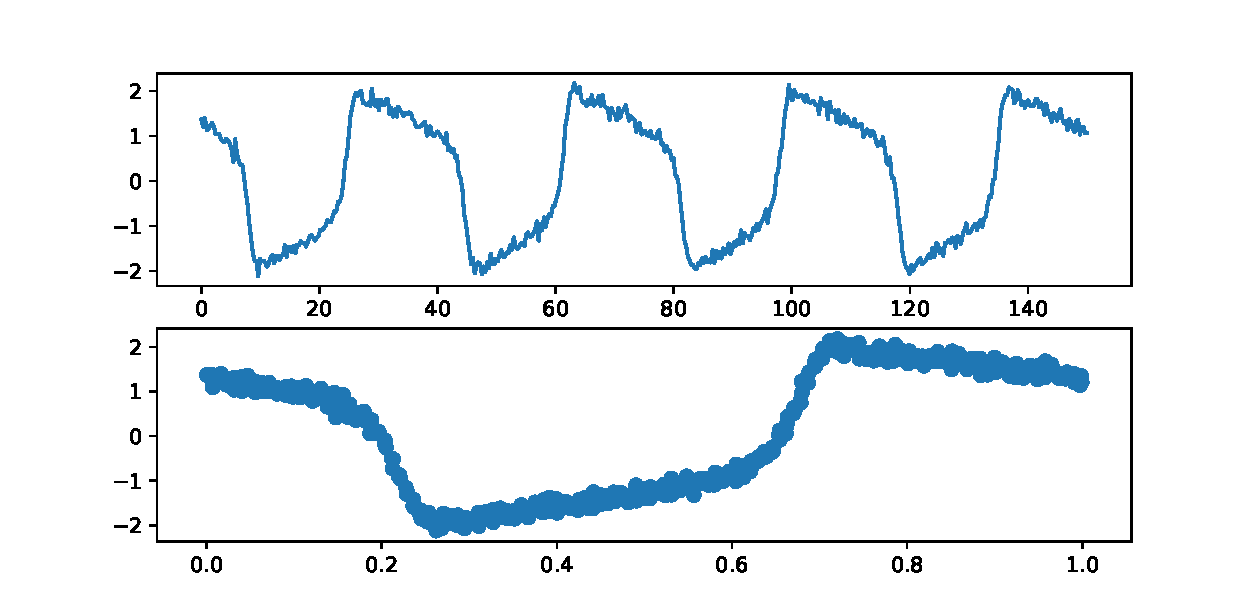
\includegraphics[width=.9\linewidth]{./period_stack2.pdf}
\end{center}
\end{frame}

\begin{frame}[label={sec:org39cd4d4}]{Fit a splines model}
\begin{itemize}[<+->]
\item Challenge: determine knot points
\begin{itemize}
\item Given a target `smoothness' \(\lambda\), we can find a knotset and LSQ BSpline curve
\item Standard method; optimizes loss \(+~\lambda~\times\) total curvature
\end{itemize}
\item Knot selection is still an unanswered problem
\begin{itemize}
\item Smoothing splines approach 1: put a knot at every datapoint
\item Smoothing splines approach 2: start off with few knots, keep adding more until we get target smoothness
\item Overparameterises -- neither of these give low-dimensional discretisation!
\end{itemize}
\item Well-chosen knot points are needed for a low-dimensional discretisation
\begin{itemize}
\item Hard to choose good knots \emph{a priori}; method 2 is automated trial and error
\item Standard methods don't give a minimal knotset
\item Hard to optimise knotsets due to lots of local minima
\end{itemize}
\item \alert{Turns out we can make a naive method, that works very well\ldots{}}
\end{itemize}
\end{frame}

\begin{frame}[label={sec:org49a670f}]{Knot fitting}
\begin{enumerate}[<+->]
\item Choose the desired number of knots
\begin{itemize}
\item A mixture of intuition and experimentation
\item Heuristic: put a knot either side of the signal `turning points'
\item Fitzhugh-Nagumo: 4 turning points, so try 8 knots
\end{itemize}
\item Choose knots at random
\item Numerically optimize the knot vector
\item Repeat steps 2,3 lots, and choose the best result
\begin{itemize}
\item Helps overcome the local minima issue
\end{itemize}
\end{enumerate}
\end{frame}

\begin{frame}[label={sec:orgffc5b4d}]{Knot fitting}
This works surprisingly well:
\begin{itemize}
\item Few knots = model quick to fit, easier to optimise
\item Nice result would be to analytically derive a LSQ fitting procedure
\end{itemize}
\vfill
For comparison\ldots{}
\begin{itemize}[<+->]
\item Bayesian automatically selects required number of knots
\begin{itemize}
\item No trial and error
\item Takes human out the loop
\end{itemize}
\item Bayesian automatically finds the best knots
\item Bayesian could overcome the period estimation problem \emph{[see later]}
\item This method gets good results much more simply
\end{itemize}
\end{frame}

\begin{frame}[label={sec:orgdc37deb}]{Smoothness fit}
   \begin{center}
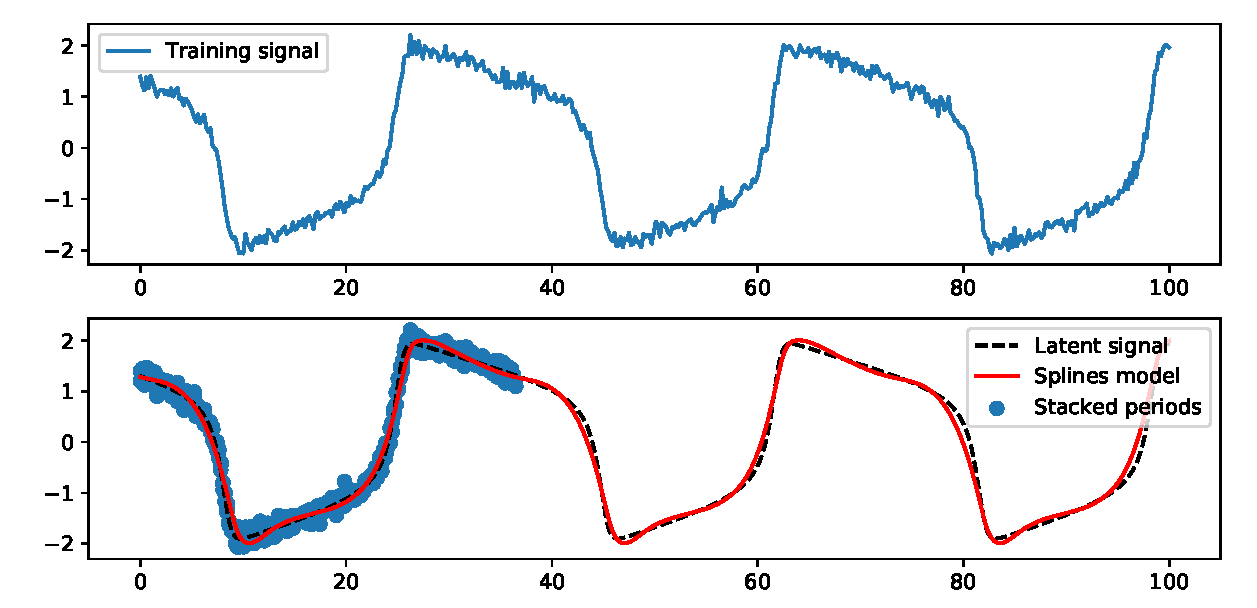
\includegraphics[width=.9\linewidth]{./fit1.pdf}
\end{center}
Smoothness = 10; 38-dimensional discretisation.
\end{frame}

\begin{frame}[label={sec:org53ba107}]{Smoothness fit}
   \begin{center}
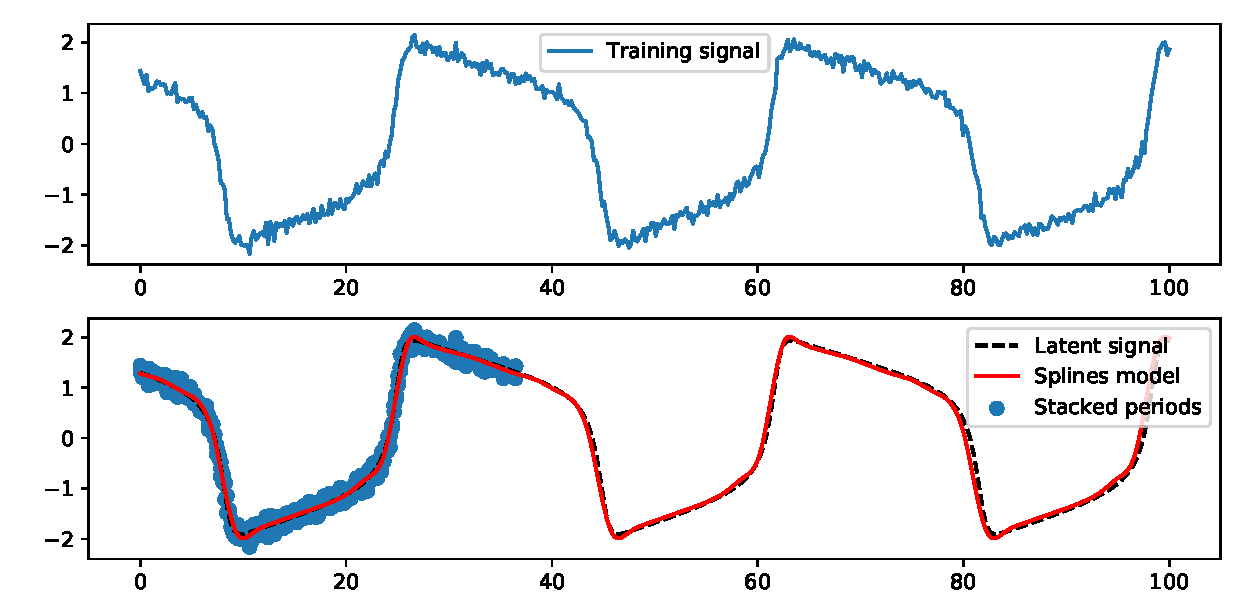
\includegraphics[width=.9\linewidth]{./fit2.pdf}
\end{center}
Smoothness = 5; 58-dimensional discretisation.
\end{frame}

\begin{frame}[label={sec:org22748d4}]{Optimizer fit}
   \begin{center}
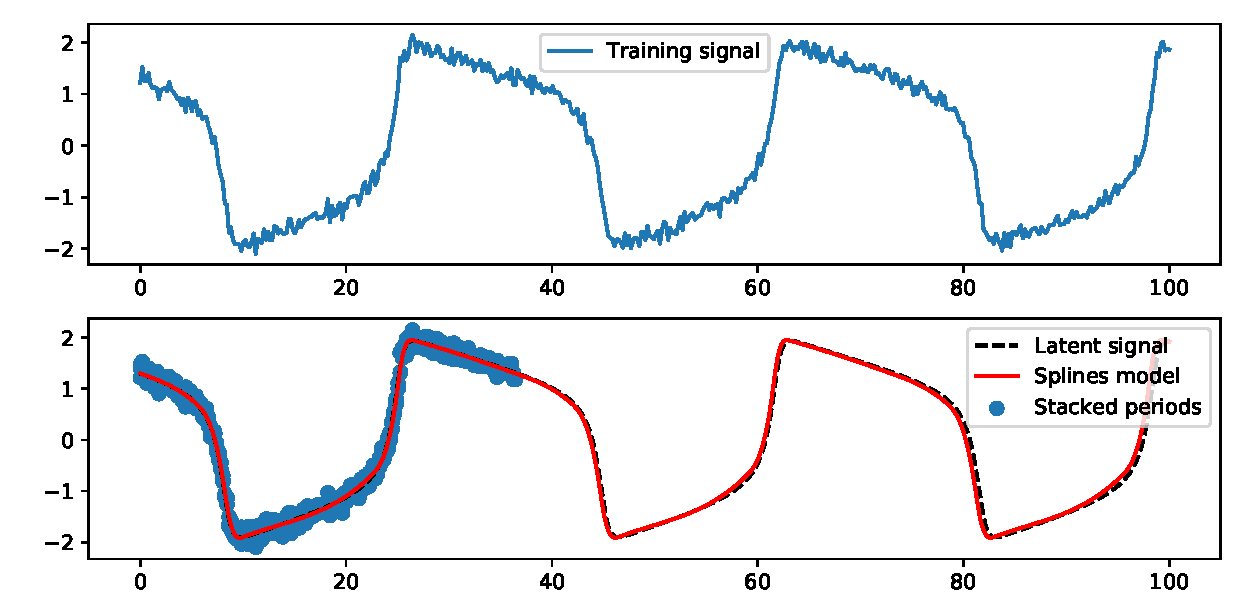
\includegraphics[width=.9\linewidth]{./fit3.pdf}
\end{center}
8 interior knots
\end{frame}

\begin{frame}[label={sec:orgcdb35c6}]{Optimizer fit}
   \begin{center}
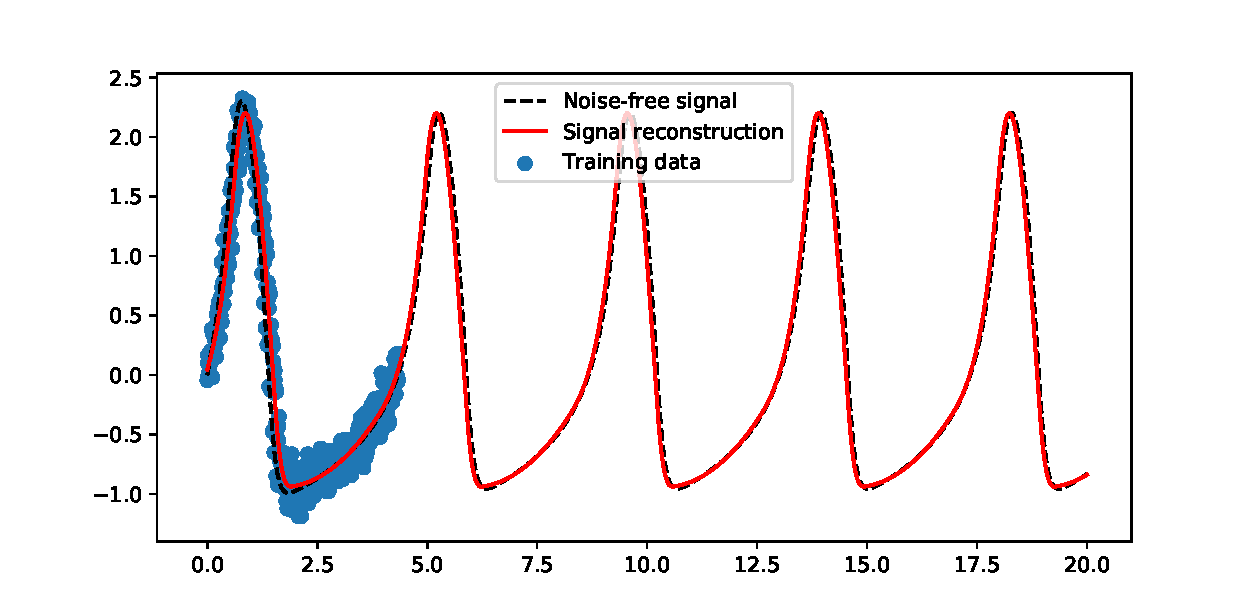
\includegraphics[width=.9\linewidth]{./HRFit.pdf}
\end{center}
Also works on more neuron-like data
\end{frame}

\begin{frame}[label={sec:org51f9f19}]{Optimizer fit}
   \begin{center}
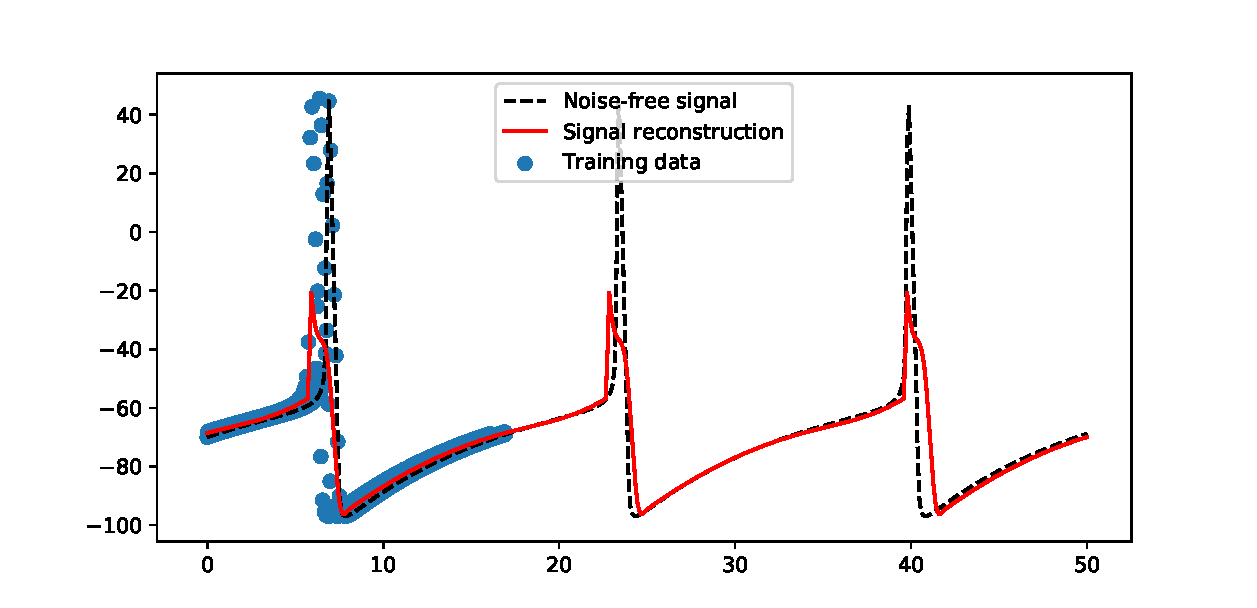
\includegraphics[width=.9\linewidth]{./HHFit.pdf}
\end{center}
Too few datapoints across the spikes
\end{frame}

\begin{frame}[label={sec:org91d14c4}]{Optimizer fit}
  \begin{center}
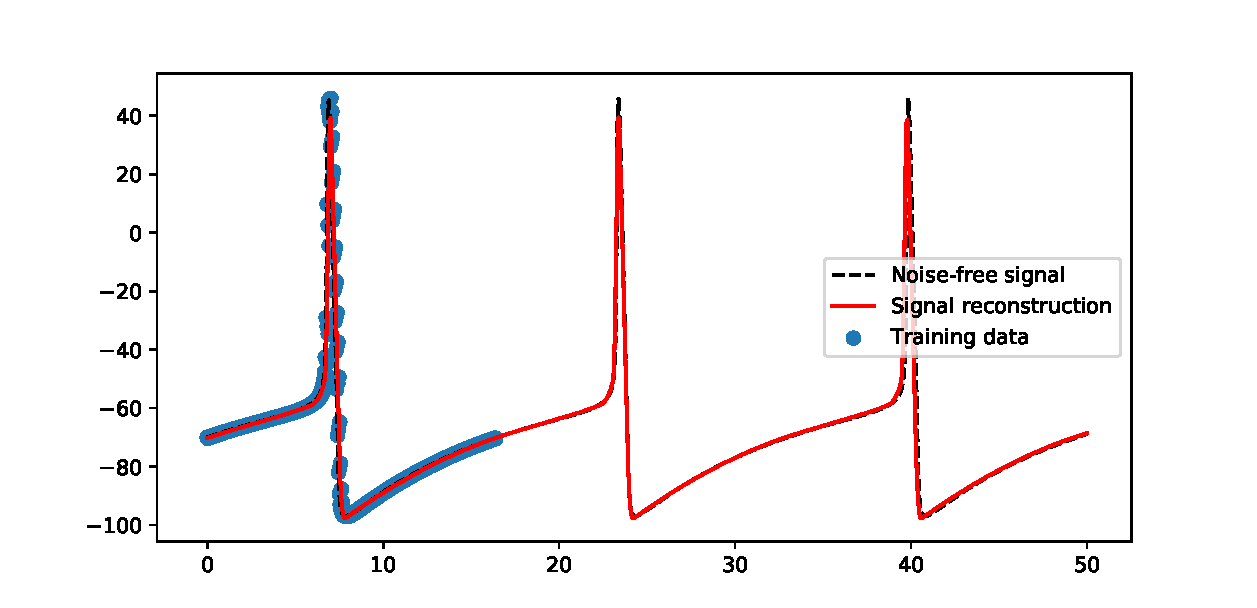
\includegraphics[width=.9\linewidth]{./HHFit2.pdf}
\end{center}
Much better!
\end{frame}


\begin{frame}[label={sec:org54d8611}]{Issue}
\begin{itemize}
\item Inaccuracies in the period will add up to a big phase shift over time
\item Bad period estimate can have disastrous results!
\end{itemize}
\end{frame}

\begin{frame}[label={sec:orgd838fee}]{The period-estimation problem}
\begin{center}
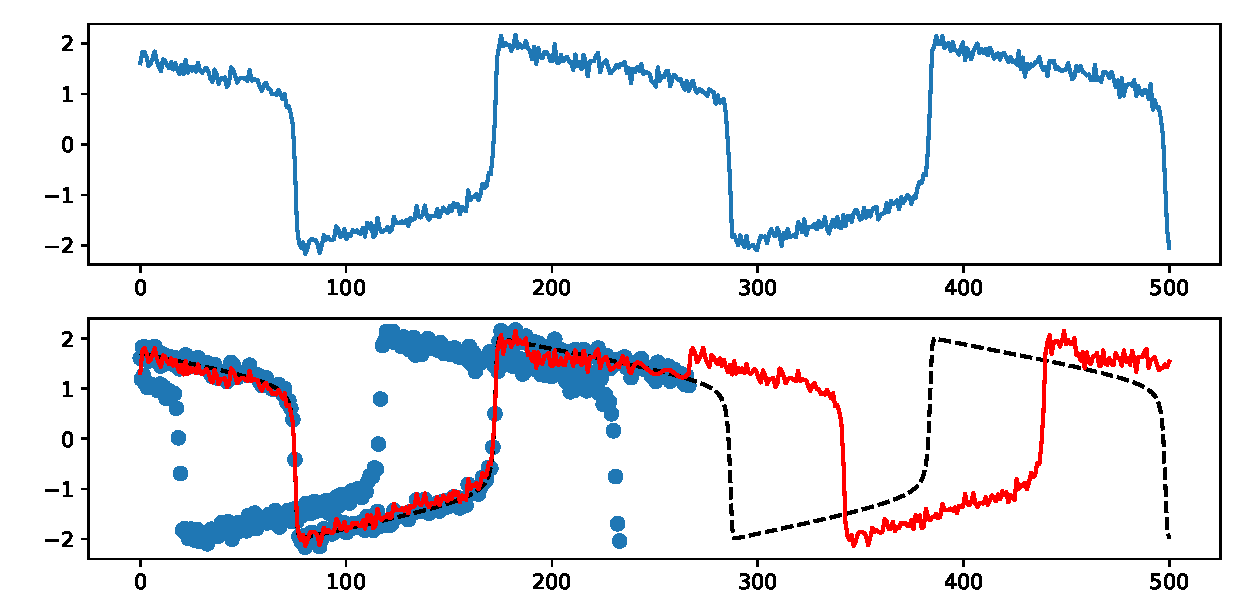
\includegraphics[width=.9\linewidth]{./brokenF0.pdf}
\end{center}
\end{frame}

\begin{frame}[label={sec:orgbf6bec0}]{The period-estimation problem}
\begin{itemize}
\item Increasing the timescale separation `squares up' the signal, but breaks F0 period estimation
\item NLS F0 estimation also uses Fourier harmonics, so breaks on the same signals Fourier discretisation would break on \emph{[only tried one test-case!]}
\item Playing with the F0 estimation parameters / methods helps with this, but adds more mysterious hyperparameters
\begin{itemize}
\item Bayesian methods also offer a way around this
\end{itemize}
\end{itemize}
\end{frame}

\section{Next steps}
\label{sec:org1f6417a}
\begin{frame}[label={sec:orge966924}]{Next steps}
\begin{itemize}
\item Keep working on paper
\item Compare reconstruction error for a given number of knots, for Fourier and splines
\item Use discretisation in CBC
\begin{itemize}
\item Treat knot positions as a fixed hyperparameter
\item BSpline coefficients become a signal discretisation
\end{itemize}
\item Mini-review knot selection methods
\begin{itemize}
\item Worth discussing the alternative methods in a paper
\end{itemize}
\end{itemize}
\end{frame}
\end{document}
